\chapter{Implementación}\label{cap6}

\newpage
\section{Entorno y Tecnologías}

Para el desarrollo e implementación del sistema, se ha seleccionado un conjunto de tecnologías de código abierto que permiten el procesamiento local de datos, garantizando la privacidad de la información y la soberanía sobre los modelos de inteligencia artificial empleados, ya que, en el caso de una empresa privada, podría preferirse no utilizar modelos externos por razones de privacidad de los datos.

\subsection{Infraestructura de Cómputo y Aceleración}
Dada la carga computacional que requiere la inferencia de modelos de lenguaje y la generación masiva de vectores, se ha hecho uso de la arquitectura de computación paralela de NVIDIA:

\begin{itemize}
    \item \textbf{NVIDIA CUDA (Compute Unified Device Architecture):} Se utiliza como plataforma de computación paralela para permitir que las librerías de \textit{deep learning} (como \texttt{PyTorch}, que sustenta a \texttt{SentenceTransformers}) y el motor \texttt{Ollama} descarguen las operaciones matemáticas pesadas en la GPU. Esto reduce drásticamente el tiempo de generación de \textit{embeddings} y aumenta la velocidad de generación de texto (\textit{tokens per second}) en comparación con el uso exclusivo de la CPU.
\end{itemize}

\subsection{Lenguaje de Programación y Entorno de Ejecución}
La implementación principal se ha realizado en \textbf{Python 3.10+}, aprovechando su maduro ecosistema de librerías para el procesamiento de lenguaje natural (NLP) y estructuras de datos complejas. El entorno de desarrollo se ha gestionado mediante un entorno virtual para asegurar la reproducibilidad de las dependencias.

\subsection{Infraestructura de Modelos de Lenguaje (LLM)}
\begin{itemize}
    \item \textbf{Ollama:} Se utiliza como motor de inferencia local para el despliegue del modelo \texttt{llama3.1:8b}. Esta herramienta permite gestionar el ciclo de vida del modelo y ajustar parámetros críticos como el \texttt{num\_ctx} (ventana de contexto), el cual se ha configurado hasta en 60,000 tokens para el procesamiento de documentos completos.
    \item \textbf{Sentence-Transformers:} Para la generación de \textit{embeddings}, se emplea el modelo \texttt{all-\allowbreak MiniLM-\allowbreak L6-v2}. Este modelo ofrece un equilibrio óptimo entre velocidad de cómputo y calidad en la representación vectorial de fragmentos de texto.
    \item \textbf{Cross-Encoders:} Se ha integrado el modelo \nolinkurl{cross-encoder/ms-marco-MiniLM-L-6-v2} para realizar tareas de \textit{reranking}. A diferencia de los \textit{bi-encoders}, este modelo analiza pares consulta-documento de forma conjunta, mejorando drásticamente la precisión del orden de relevancia final.
\end{itemize}

\subsection{Procesamiento de Documentos y Grafos}
\begin{itemize}
    \item \textbf{PyMuPDF (fitz):} Librería de alto rendimiento utilizada para la manipulación de archivos PDF. Es la pieza clave para extraer metadatos, identificar hipervínculos internos y obtener las coordenadas de los cuadros de texto necesarias para inferir la jerarquía.
    \item \textbf{NetworkX:} Librería especializada en el estudio de redes complejas. Se utiliza para construir el grafo dirigido (\texttt{DiGraph}) donde cada nodo representa una sección del documento y las aristas definen relaciones jerárquicas, secuenciales o semánticas.
    \item \textbf{Rank-BM25:} Implementación del algoritmo de relevancia \textit{Best Matching 25}. Se integra en el sistema de búsqueda híbrida para complementar la búsqueda vectorial con coincidencias exactas de términos clave.
\end{itemize}

\subsection{Otras Librerías de Apoyo}
\begin{itemize}
    \item \textbf{TheFuzz:} Utilizada para el \textit{fuzzy matching} de títulos de secciones, permitiendo que el sistema sea resiliente a pequeñas variaciones de formato o errores de extracción.
    \item \textbf{Tiktoken:} Herramienta de \textit{tokenización} utilizada para contabilizar con precisión el volumen de información enviado al modelo y prevenir el desbordamiento de la ventana de contexto.
    \item \textbf{Matplotlib:} Empleada para la generación de las representaciones visuales de los subgrafos de consulta, facilitando la auditoría del proceso de recuperación.
\end{itemize}

\newpage
\section{Procesamiento de Documentos y Extracción Estricta}
El sistema se ha diseñado bajo una arquitectura modular donde la integridad de la estructura jerárquica del documento es el pilar fundamental. A continuación, se detallan los algoritmos y procesos técnicos que permiten la transformación de documentos PDF en una base de conocimiento funcional para RAG.
La lógica de extracción, implementada en el módulo \texttt{chunk\_extractor.py}, trasciende la simple recuperación de texto plano para enfocarse en la topología del documento.

\subsection{Algoritmo de Extracción y Limpieza}
La función \texttt{extract\_links\_with\_detailed\_debug} actúa como el punto de entrada. Utiliza la librería \texttt{PyMuPDF} para identificar metadatos de navegación. El proceso sigue un flujo de decisión:
\begin{itemize}
    \item \textbf{Detección de Hipervínculos:} Se utiliza \texttt{page.get\_links()} para extraer anotaciones de salto interno. Se recupera el texto contenido en el rectángulo del enlace (\texttt{textbox}) y se vincula a su página de destino (\texttt{target\_page}).
    \item \textbf{Filtro de Márgenes:} Mediante \texttt{get\_page\_margins}, se define un área de interés que excluye el 10\% de cada borde de la página. El objetivo es reducir elementos de ruido como números de página, encabezados y pies de página que podrían contaminar la calidad de los \textit{embeddings}.
\end{itemize}

A continuación se ilustra gráficamente el filtro de márgenes. En los tipos de archivo para los que se ha especializado el sistema, es habitual encontrar texto repetido, títulos de sección, firmas digitales u otros contenidos en las zonas superior, inferior o lateral de la página; por ejemplo:

\begin{figure}[H]
    \centering
    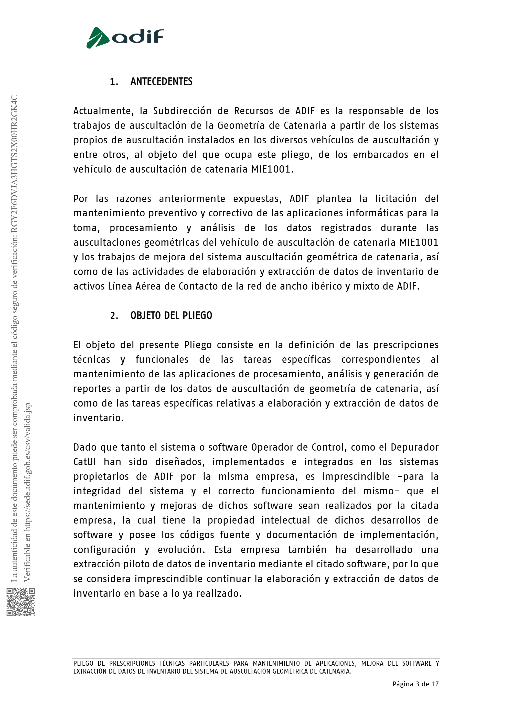
\includegraphics[width=0.8\textwidth]{images/PliegoSinMargenes.png}
    \caption{Página de un pliego técnico de ADIF como ejemplo de contenido en márgenes}
    \label{fig:PliegoConBordes}
\end{figure}

Como se aprecia en la imagen, existe texto tanto en el margen izquierdo como en el superior. Aunque individualmente puede parecer escaso, en documentos de cientos de páginas representa una cantidad considerable de contenido irrelevante; tras aplicar el filtro, el área efectiva queda reducida a lo siguiente:

\begin{figure}[H]
    \centering
    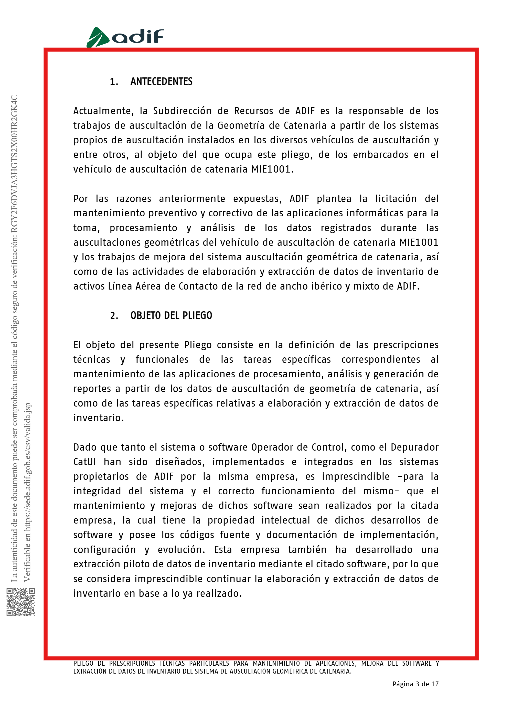
\includegraphics[width=0.8\textwidth]{images/PliegoMargenesQuitados.png}
    \caption{La parte dentro del rectángulo rojo representa lo que se verá}
    \label{fig:PliegoMargenes}
\end{figure}

\newpage

\subsection{Reconstrucción Jerárquica mediante Posición X}
En la función \texttt{organizar\_indice}, se implementa una lógica de inferencia para documentos que carecen de una numeración explícita (ej. 1.1, 1.2). El sistema utiliza la propiedad \texttt{X} (posición horizontal) de la coordenada de origen del enlace:
\begin{itemize}
    \item \textbf{Indentación:} Si un elemento presenta una coordenada \texttt{X} significativamente mayor que el anterior, se clasifica automáticamente como una subsección (\textit{hijo}).
    \item \textbf{Parentesco:} El sistema asigna un ID jerárquico y vincula el nodo a su padre más cercano en la pila de procesamiento, permitiendo reconstruir el árbol documental completo.
\end{itemize}

\newpage
\section{Arquitectura del Grafo de Conocimiento (NetworkX)}

Tras la fase de segmentación y extracción, los fragmentos de información (\textit{chunks}) no se almacenan como elementos aislados, sino que se integran en una estructura de grafo dirigido ($\texttt{DiGraph}$) utilizando la librería \texttt{NetworkX}. Esta arquitectura es la que habilita la capacidad de \textbf{GraphRAG}, permitiendo realizar búsquedas que respetan tanto la jerarquía como la semántica del documento original.

\subsection{Modelado de Nodos y Atributos}
Cada nodo en el grafo representa una unidad de información (sección o subsección). Para garantizar la trazabilidad y la eficacia en la recuperación, a cada nodo se le asignan los siguientes atributos técnicos:
\begin{itemize}
    \item \textbf{Content:} El cuerpo de texto normalizado y limpio.
    \item \textbf{Level:} Profundidad jerárquica (ej. Nivel 0 para capítulos, Nivel 1 para secciones).
    \item \textbf{Page Range:} Tupla con la página de inicio y fin para permitir la citación precisa en la respuesta final.
    \item \textbf{Vector Embedding:} Representación numérica del contenido generada mediante el modelo \texttt{all-\allowbreak MiniLM-\allowbreak L6-v2}.
\end{itemize}

\subsection{Tipología de Aristas y Relaciones Multimodales}
La innovación del sistema reside en la coexistencia de diferentes tipos de aristas, lo que permite navegar el documento de forma no lineal:
\begin{itemize}
    \item \textbf{Aristas Jerárquicas:} Definen la relación \textit{Padre-Hijo}. Se crean automáticamente basándose en el ID de la sección y la indentación detectada en el PDF.
    \item \textbf{Aristas Secuenciales:} Conectan fragmentos adyacentes dentro del flujo de lectura original, permitiendo al sistema recuperar el contexto inmediato (anterior y posterior) de un dato específico.
    \item \textbf{Aristas Semánticas:} Implementadas mediante el método \texttt{add\_semantic\_edges}. Se calculan relaciones de similitud de coseno entre todos los nodos del grafo; si la similitud supera un umbral de $0.65$, se establece un vínculo bidireccional. Esto permite conectar conceptos relacionados que se encuentran en capítulos distantes del documento.
\end{itemize}

\subsection{Algoritmo de Propagación de Relevancia (Family Scores)}
Para mitigar el problema de los fragmentos con poco texto que carecen de peso semántico por sí mismos, se ha implementado la técnica de \textbf{Propagación Familiar}. El sistema ajusta la relevancia de un nodo en función de su entorno:

\begin{equation}
Score_{final}(n) = (Score_{similitud}(n) \times w_{1}) + (\max(Score_{familia}(n)) \times w_{2})
\end{equation}

Donde $w_{1}$ y $w_{2}$ son pesos configurables (con un valor de $0{,}5$ en la configuración empleada). Esta lógica favorece que, si una sección secundaria es relevante, su sección ``padre'' (que contiene el contexto general) también sea recuperada para su inclusión en el \textit{prompt} del modelo.

\begin{figure}[h]
    \centering
    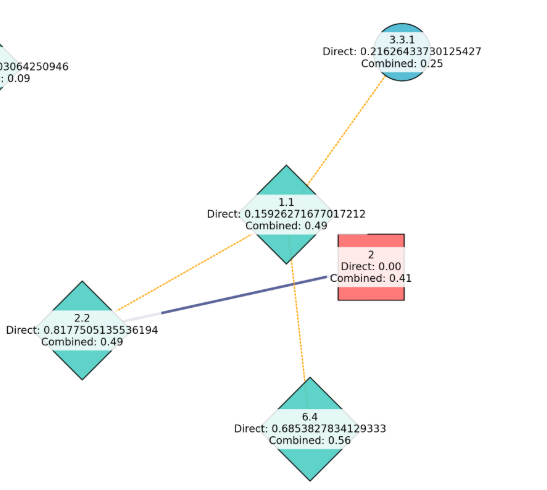
\includegraphics[width=0.8\textwidth]{images/ConexionSemantico_Jerarquico.png}
    \caption{Gráfico con un nodo central conectado mediante similitud familiar (azul) y semántica (amarilla)}
    \label{fig:ConexionSemantico_Jerarquico}
\end{figure}

\newpage
\subsection{Recuperación de Contexto mediante Centralidad}
Finalmente, el sistema utiliza algoritmos de centralidad de grafos para seleccionar la información más densa en contenido. Al realizar una consulta, el sistema extrae un subgrafo de interés y aplica \textbf{PageRank} para identificar qué nodos actúan como ejes centrales de información dentro de la selección. La función \texttt{get\_optimal\_context} filtra y ordena estos nodos, limitando la cantidad de texto enviado al LLM para no saturar su ventana de contexto y favoreciendo una mayor representatividad del documento dentro del presupuesto de tokens disponible.

\begin{figure}[h]
    \centering
    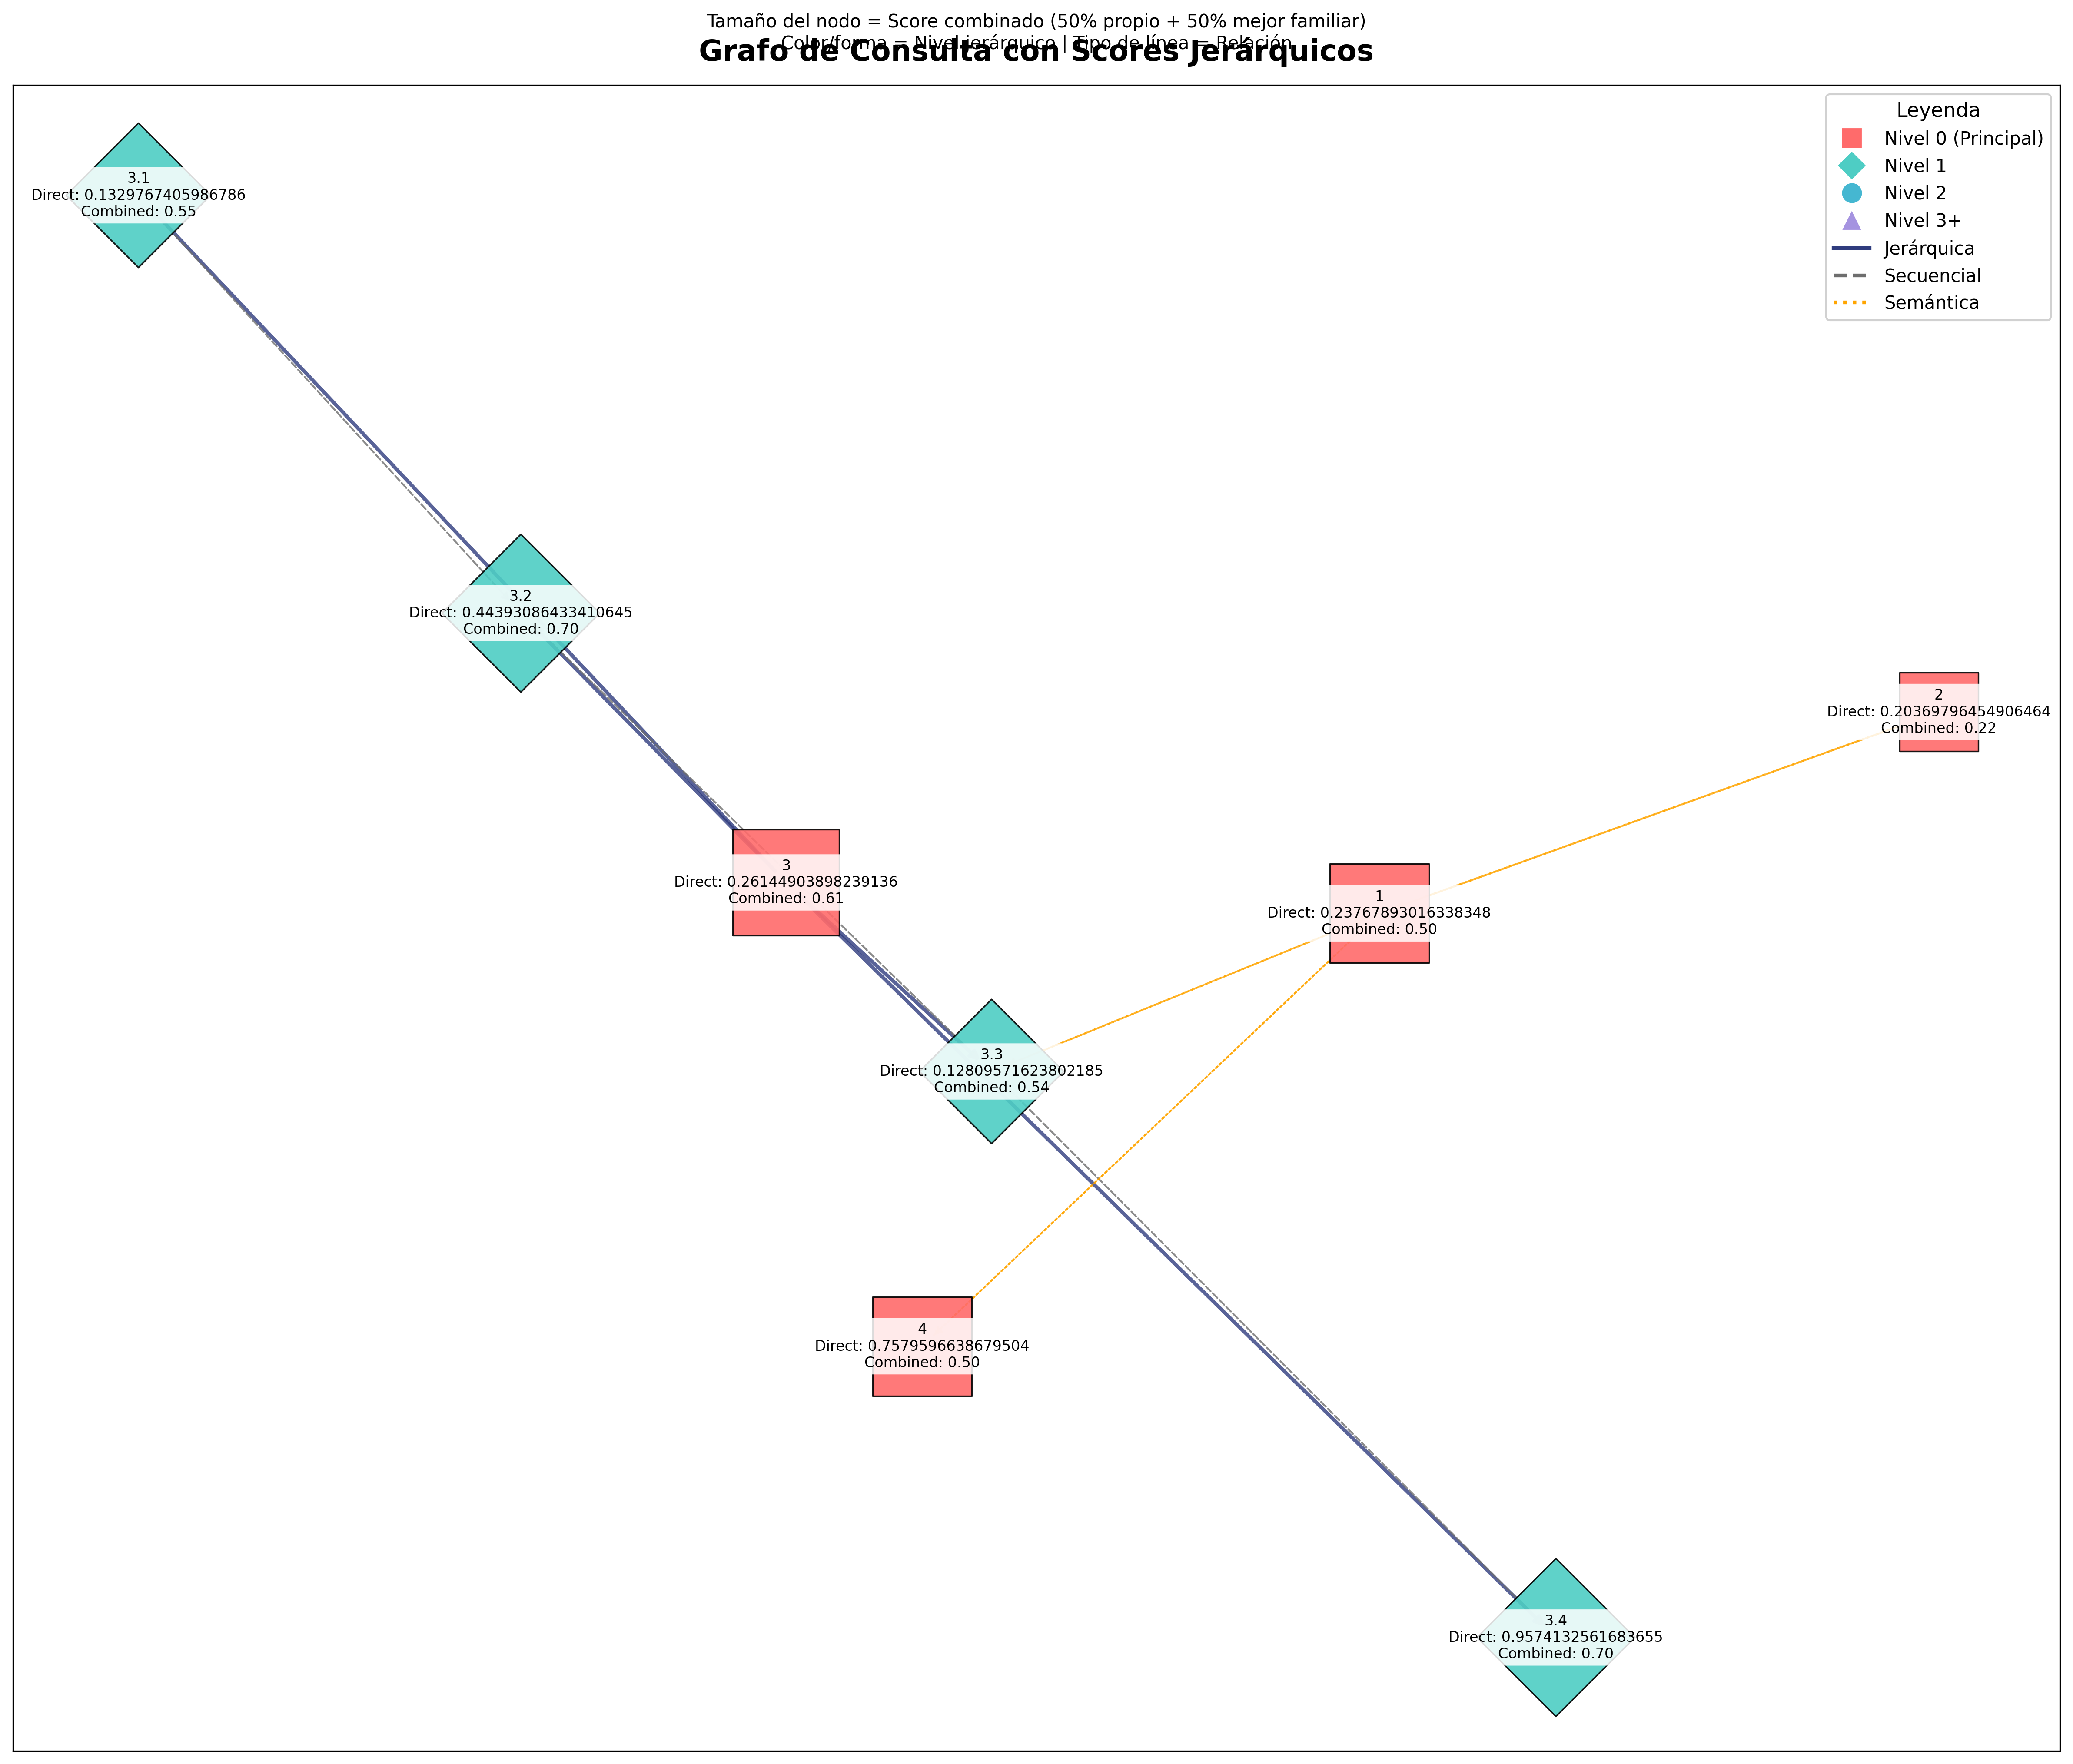
\includegraphics[width=1\textwidth]{images/graficoQuery.png}
    \caption{Ejemplo de gráfico generado}
    \label{fig:GraficoGenerado}
\end{figure}

\newpage
\section{Pipeline de Búsqueda Híbrida y Reranking}

Para maximizar la precisión en la recuperación de información, el sistema implementa un flujo de trabajo multietapa que combina algoritmos de búsqueda léxica y semántica, culminando en un proceso de re-clasificación profunda (\textit{reranking}). Este enfoque mitiga las limitaciones individuales de cada técnica, como el ruido semántico o la incapacidad de capturar sinónimos.

\subsection{Estrategia de Búsqueda Híbrida (BM25 + Embeddings)}
La función \texttt{query\_chunks\_hybrid} coordina la recuperación inicial utilizando dos motores paralelos:
\begin{itemize}
    \item \textbf{Recuperación Léxica (BM25):} Mediante la librería \texttt{Rank-BM25}, el sistema analiza la coincidencia exacta de términos clave. Esto es vital para identificar códigos técnicos, normativas o términos específicos que los modelos de \textit{embeddings} podrían diluir en el espacio vectorial.
    \item \textbf{Recuperación Semántica:} Se utiliza el modelo \texttt{all-\allowbreak MiniLM-\allowbreak L6-v2} para calcular la similitud del coseno entre la consulta y los fragmentos. A diferencia de un RAG estándar, se aplica un proceso de \textbf{sub-chunking semántico} mediante \texttt{RecursiveCharacterTextSplitter}, dividiendo cada sección en micro-fragmentos de 100 caracteres para localizar respuestas precisas dentro de secciones extensas.
\end{itemize}

\subsection{Estrategia de Doble Granularidad: Sub-chunking Semántico}
Una de las innovaciones clave en la implementación del buscador es la superposición de dos niveles de granularidad. Mientras que el grafo gestiona unidades lógicas (secciones), la búsqueda vectorial opera sobre micro-fragmentos generados mediante \texttt{RecursiveCharacterTextSplitter}:
\begin{itemize}
    \item \textbf{Nivel Macro (Grafo):} Proporciona el contexto estructural y las relaciones de parentesco.
    \item \textbf{Nivel Micro (Sub-chunks):} Se generan fragmentos de 100 caracteres con un solapamiento (\textit{overlap}) de 20 caracteres. Esto permite que el modelo de \textit{embeddings} capture la semántica exacta de una frase técnica sin la "dilución" que ocurre cuando se vectorizan párrafos muy extensos.
\end{itemize}
Esta aproximación permite que, ante una consulta específica, el sistema localice el sub-chunk exacto y, gracias a la estructura de grafo, recupere automáticamente la sección completa a la que pertenece.

\subsection{Ponderación de Resultados y Fusión}
Los resultados de ambos motores se normalizan y combinan. El sistema otorga un peso del $67,5\%$ a la similitud semántica y un $32,5\%$ a la puntuación BM25. Esta ponderación busca que la respuesta tenga sentido conceptual sin sacrificar la precisión en la recuperación de términos clave utilizados por el usuario.

\subsubsection{Justificación de Umbrales y Ponderaciones}
Los valores de configuración se han ajustado tras una fase de pruebas empíricas:
\begin{itemize}
    \item \textbf{Umbral Semántico ($\tau = 0.65$):} Se seleccionó para evitar el fenómeno de ``grafo denso'', donde demasiadas conexiones semánticas irrelevantes difuminan la estructura jerárquica.
    \item \textbf{Ponderación Híbrida (67.5\% Vectorial / 32.5\% BM25):} Este equilibrio favorece la comprensión de conceptos sobre la coincidencia de palabras, pero mantiene la capacidad de encontrar términos técnicos específicos (códigos de error, nombres de funciones) que el motor léxico detecta con mayor fiabilidad.
\end{itemize}

\subsection{Re-clasificación Profunda mediante Cross-Encoder}
Debido a que los modelos de \textit{bi-encoders} (usados para los \textit{embeddings}) procesan la consulta y el documento de forma independiente, pueden perder matices relacionales. Para resolver esto, se implementa una etapa de \textbf{Reranking} con el modelo \nolinkurl{cross-encoder/ms-marco-MiniLM-L-6-v2}:
\begin{itemize}
    \item El sistema toma los mejores candidatos de la búsqueda híbrida y los somete a una comparación por pares (consulta, fragmento).
    \item El \textit{Cross-Encoder} genera una puntuación de relevancia mucho más precisa, ya que analiza la interacción completa entre las palabras de la pregunta y el contenido del fragmento.
    \item Solo aquellos fragmentos que superan el umbral de confianza tras el re-rankeo (\texttt{min\_similarity}) son considerados para la fase final de generación.
\end{itemize}

\subsection{Integración de Contexto Jerárquico}
Una vez obtenidos los fragmentos finales, el sistema no los entrega al LLM de forma desordenada. Se invoca a \texttt{get\_context\_with\_hierarchy} para reconstruir la estructura documental: los fragmentos se agrupan por documento de origen y se ordenan según su \texttt{section\_id}. Esto permite que el modelo de lenguaje reciba un contexto coherente, respetando el orden lógico del autor original, lo que reduce drásticamente las alucinaciones en la respuesta final.

\newpage
\section{Orquestación y Agentes Inteligentes}

El sistema no se limita a una recuperación estática de datos, sino que implementa una capa de inteligencia agéntica que coordina el flujo de trabajo basándose en la intención del usuario. Esta lógica se centraliza en la clase \texttt{SmartDocumentProcessor}.

\subsection{Agente de Selección de Estrategia (PARTIAL vs FULL)}
El primer componente crítico es el \texttt{DocumentStrategyAgent}. Su función es analizar la consulta del usuario y los metadatos de los documentos cargados para decidir la ruta de procesamiento óptima.

Mediante la función \texttt{analyze\_query}, se envía un \textit{prompt} estructurado al modelo \texttt{llama3.1:8b} que incluye el número de documentos y su extensión media. El agente clasifica la consulta en dos categorías:
\begin{itemize}
    \item \textbf{PARTIAL (RAG approach):} Seleccionada cuando la consulta busca datos específicos o secciones concretas, activando el motor de búsqueda en grafos.
    \item \textbf{FULL (Full Document):} Seleccionada para tareas de síntesis global, comparaciones transversales o resúmenes de documentos completos. En este caso, el sistema omite el filtrado y utiliza una ventana de contexto extendida de hasta 60,000 tokens.
\end{itemize}

\subsection{Control de Saturación y Ventana de Contexto}
Dado que el modelo \texttt{llama3.1:8b} posee límites físicos de memoria, la implementación incorpora un gestor de tokens basado en \texttt{tiktoken}. Antes de realizar la llamada a la API local de Ollama, el sistema ejecuta:
\begin{enumerate}
    \item \textbf{Cómputo de Presupuesto:} Se calcula el total de tokens del \textit{prompt} del sistema y la consulta.
    \item \textbf{Recorte Dinámico:} Si el contexto recuperado (especialmente en modo \texttt{FULL}) supera el límite de seguridad (configurado al 90\% del \texttt{num\_ctx}), el sistema prioriza los nodos con mayor puntuación de PageRank y cercanía semántica, descartando los fragmentos menos informativos para evitar errores de inferencia.
\end{enumerate}

\subsection{Optimización Dinámica de Consultas}
Incluso en el modo RAG, las preguntas de los usuarios suelen contener ruido lingüístico que dificulta la coincidencia semántica. Para solventar esto, se ha implementado el método \texttt{generate\_opti\-mized\_query}.

Este agente actúa como un purificador semántico, transformando instrucciones complejas (ej. ``Podrías buscar y explicarme detalladamente los requisitos de...'') en vectores de búsqueda esenciales (ej. ``Requisitos de...''). Esta reducción de dimensionalidad en la consulta original mejora significativamente la precisión de los \textit{scores} directos en el grafo de \texttt{NetworkX}.

\subsection{Gestión de Respuestas Individuales y Consolidadas}
El procesador permite al usuario alternar dinámicamente entre dos modos de respuesta mediante la interfaz \texttt{interactive\_chat}:
\begin{itemize}
    \item \textbf{Modo 1 (Individual):} Ejecuta una instancia de consulta por cada documento de forma aislada, útil para comparaciones paralelas.
    \item \textbf{Modo 2 (Consolidado):} Unifica los contextos recuperados de todos los documentos en un único \textit{prompt}, permitiendo al LLM identificar contradicciones o sinergias entre las fuentes.
\end{itemize}

\subsection{Observabilidad y Visualización}
Finalmente, la lógica de implementación incluye un mecanismo de depuración visual. Si se activa el parámetro \texttt{visualize}, el sistema utiliza \texttt{Matplotlib} para volcar el subgrafo de consulta en un archivo PNG. Esto permite verificar físicamente si la propagación de relevancia familiar y las aristas semánticas están capturando los nodos correctos antes de la generación de la respuesta.

\newpage
\section{Interfaz y Control del Chat Interactivo}

La interacción final con el sistema se realiza a través de un bucle de control robusto implementado en el método \texttt{interactive\_chat}. Este componente no solo actúa como interfaz, sino como el gestor de estados que coordina todas las tecnologías descritas anteriormente.

\subsection{Gestión de Estados y Modos de Operación}
El sistema mantiene un estado interno que permite al usuario modificar el comportamiento de la recuperación en tiempo real sin necesidad de reiniciar el procesamiento de los documentos. El flujo lógico se gestiona mediante comandos de control:
\begin{itemize}
    \item \textbf{Selección de Modo:} El usuario puede alternar entre el procesamiento individual (\textit{Modo 1}) y el consolidado (\textit{Modo 2}), lo que redirige la consulta hacia \texttt{generate\_graph\_responses} o \texttt{generate\_consolidated\_graph\_response} respectivamente.
    \item \textbf{Control de Observabilidad:} Mediante los comandos \texttt{visualizar si/no}, se activa el motor de renderizado de \texttt{NetworkX} y \texttt{Matplotlib} para generar la representación gráfica de los nodos consultados.
\end{itemize}

\subsection{Ciclo de Retroalimentación y Generación}
Para cada consulta ingresada, el sistema ejecuta un hilo de ejecución secuencial:
\begin{enumerate}
    \item \textbf{Tokenización Preventiva:} Se utiliza \texttt{tiktoken} para validar que el contexto jerárquico recuperado no exceda los límites físicos del modelo seleccionado, con el fin de reducir el riesgo de truncamiento y favorecer la estabilidad de la respuesta.
    \item \textbf{Inyección de Prompt Estructurado:} El sistema construye un \textit{prompt} final que incluye instrucciones de comportamiento (ej. ``señala contradicciones'', ``menciona fuentes'') junto con el contexto filtrado por los \textit{scores} de familia y centralidad.
    \item \textbf{Presentación de Resultados:} La respuesta se presenta desglosada por documento de origen, incluyendo metadatos sobre la página y la sección, lo que permite al usuario final realizar una validación cruzada inmediata con el PDF original.
\end{enumerate}

\subsection{Punto de Entrada del Sistema (Main)}
La ejecución principal en la función \texttt{main} coordina la inicialización de \texttt{PDFRAG\-System\-With\-NetworkX}, cargando todos los archivos desde un directorio específico y delegando la lógica de decisión al \texttt{Smart\-Document\-Processor}. Esta arquitectura está diseñada para escalar a múltiples documentos manteniendo una latencia de respuesta razonable gracias a la aceleración por hardware (CUDA) detallada en la sección 6.1.

\newpage
\section{Gestión de Errores y Resiliencia del Sistema}
Para garantizar la robustez operativa, se han implementado controles específicos ante situaciones críticas identificadas durante las pruebas:

\begin{itemize}
    \item \textbf{PDF sin Estructura o Corruptos:} Si la extracción mediante hipervínculos falla, la función \texttt{extract\_links\_with\_detailed\_debug} conmuta automáticamente a un modo de búsqueda por patrones (\textit{fallback}). En caso de documentos escaneados sin capa de texto (OCR), el sistema notifica la incapacidad de lectura en lugar de generar una respuesta vacía o errónea.
    \item \textbf{Control de Alucinaciones por Falta de Contexto:} Mediante el ajuste del parámetro \texttt{min\_thres\-hold}, si ningún nodo del grafo supera el umbral de similitud semántica o léxica, el sistema está instruido para responder que la información no está disponible en los documentos cargados, evitando que el LLM genere información falsa.
    \item \textbf{Consultas Fuera de Dominio:} El \texttt{DocumentStrategyAgent} actúa como primer filtro. Si la consulta no tiene relación con el contenido documental (ej. una pregunta de cultura general), el razonamiento del agente permite abortar la búsqueda en el grafo, ahorrando recursos de computación y manteniendo el enfoque en el caso de uso.
    \item \textbf{Gestión de Desbordamiento de Contexto:} El uso de \texttt{tiktoken} permite realizar un recorte preventivo en la fase de construcción del \textit{prompt}. Si el volumen de contexto recuperado por el grafo excede la capacidad del modelo, se eliminan los nodos con menor puntuación de centralidad (\textit{PageRank}) hasta cumplir con el límite de seguridad del motor de inferencia.
\end{itemize}
